\documentclass{article}

% if you need to pass options to natbib, use, e.g.:
% \PassOptionsToPackage{numbers, compress}{natbib}
% before loading nips_2017
%
% to avoid loading the natbib package, add option nonatbib:
% \usepackage[nonatbib]{nips_2017}

\usepackage{graphicx}
\usepackage{amsmath}

\usepackage{bm}

\graphicspath{ {../figs/}}

\usepackage[final]{report}

% to compile a camera-ready version, add the [final] option, e.g.:
% \usepackage[final]{nips_2017}

\usepackage[utf8]{inputenc} % allow utf-8 input
\usepackage[T1]{fontenc}    % use 8-bit T1 fonts
\usepackage{hyperref}       % hyperlinks
\usepackage{url}            % simple URL typesetting
\usepackage{booktabs}       % professional-quality tables
\usepackage{amsfonts}       % blackboard math symbols
\usepackage{nicefrac}       % compact symbols for 1/2, etc.
\usepackage{microtype}      % microtypography

\DeclareMathOperator*{\argmax}{arg\,max} % thin space, limits underneath in displays

\title{Gaussian process classifiers and CNN uncertainty}

% The \author macro works with any number of authors. There are two
% commands used to separate the names and addresses of multiple
% authors: \And and \AND.
%
% Using \And between authors leaves it to LaTeX to determine where to
% break the lines. Using \AND forces a line break at that point. So,
% if LaTeX puts 3 of 4 authors names on the first line, and the last
% on the second line, try using \AND instead of \And before the third
% author name.

\author{
  Sebastian Borgeaud dit Avocat \\
  \texttt{spb61@cam.ac.uk} \\ \\
  LE49 - Probabilistic Machine Learning Project
}

\begin{document}
%\nipsfinalcopy is no longer used

\maketitle

\begin{abstract}
  The abstract paragraph should be indented \nicefrac{1}{2}~inch
  (3~picas) on both the left- and right-hand margins. Use 10~point
  type, with a vertical spacing (leading) of 11~points.  The word
  \textbf{Abstract} must be centered, bold, and in point size 12. Two
  line spaces precede the abstract. The abstract must be limited to
  one paragraph.
\end{abstract}

\section{Introduction}
Model uncertainty is often of crucial importance.

Softmax output does not give model confidence, maybe show the example used by Yarin Gal.

With model uncertainty it is possible to treat uncertain inputs and special cases explicitly. Example if model uncertainty is high we might decide to pass the input to a human for classification.

Another example is in Reinforcement learning: with uncertainty a RL agent can decided when to explore and when to exploit in an environment. With principled uncertainty for the agent's Q-value function, it can learn much faster using techniques such as Thompson sampling.

Yarin Gal shows how dropout in neural networks can be interpreted as a Bayesian approximantion of a Gaussian Process.
\subsection{Convolutional neural networks \cite{DBLP:journals/corr/GuWKMSSLWW15} (ADD MORE CITATIONS)}
Convolutional neural networks (CNNs) were originally inspired by biological processes. They have become standard in many deep learning applications, especially in image processing or vision tasks. A convolutional neural network is a type of feedforward neural network, typically consisting of convolution layers, pooling layers and fully connected layers:
\begin{itemize}
	\item \textbf{Convolution layers} are composed of  several 	convolution kernels each computing a different feature map. The output feature maps are obtained by convolving the input with the convolution kernel and then applying an element-wise nonlinearity. Mathematically, the feature value $z_{i,j,k}^l$ at location $(i,j)$ of the $k\textsuperscript{th}$ feature map in the $l\textsuperscript{th}$ layer is computed as:
	\[z_{i,j,k}^l = {\mathbf{w}_k^l}^T \mathbf{x}_{i,j}^l + b_k^l\]
	where  $\mathbf{w}_k^l$ and $b_k^l$ are the weight and bias vectors for the $k\textsuperscript{th}$ convolution kernel in the $l\textsuperscript{th}$ layer and $\mathbf{x}_{i,j}^l$ is the input patch centered around $(i,j)$ in the $l\textsuperscript{th}$ layer. The ouput value is computed by apply a nonlinearity $a(\cdot)$ point-wise:
	\[x_{i,j,k}^{(l+1)} = a(z_{i,j,k}^l) \]

	\item \textbf{Pooling layers} aim to achieve shift-invariance and reduce the number of parameters in the network by reducing the resolution of the feature maps. The pooling layer operates on each feature map independently. Mathematically, the output of a pooling layer with pooling operation $\textrm{pool}(\cdot)$ is given by 
	\[ y_{i,j,k}^l = \textrm{pool}(x^l_{m,n,k}), \forall (m,n) \in \mathcal{R}_{i,j}\]
	where $\mathcal{R}_{i,j}$ is a local neighbourhood around $(i,j)$. Typically, the pooling operation computes the average or the maximum.
	
	\item \textbf{Fully connected layers} connect every neuron in the previous layer to single neuron in the current layer. Fully connected layers are the layers used in standard neural networks. Mathematically, the output of a fully connected layer is given by:
	\[ x^{(l+1)}_i = a\Big(\big( \sum_j w_{i,j}^l x^l_j \big) + b^l_i\big)\]
	where $a(\cdot)$ is a nonlinearity, $w_{i,j}^l$ is the weight connecting neuron $j$ in the $l\textsuperscript{th}$ layer to neuron $i$ in layer $(l+1)\textsuperscript{th}$, and $b_i^l$ is the bias weight for neuron $i$.
\end{itemize}
Optimising a convolutional neural network is done in the same way as optimising standard neural networks. A differentiable loss function is computed for the training examples (often done in batches) and the gradients w.r.t.\ the weights of the network are computed. Using these gradients, the weights are updated in a gradient descent step. Typically, more complex update rule that take into account change momentum (e.g. Adam \cite{adam}) are used as they converge faster to a local minimum. 

\subsection{Gaussian processes}
Formally, a Gaussian Process is defined as a collection of random variables, any finite number of which have (consistent) joint Gaussian distributions. A Gaussian process therefore defines a distribution over functions and is fully specified by a mean function $m(x)$ and a covariance function $k(x, x')$. Write $f \sim \mathcal{GP}(m, k)$ meaning $f$ is distributed as a GP with mean $m$ and covariance $k$.

Using the GP we can draw samples from the function for any finite number $n$ of locations. Given locations $\mathbf{x} = [x_1, \dots, x_n]$, first compute $\mu_i = m(x_i)$, $\Sigma_{i,j} = k(x_i, x_j)$. We can then sample a vector from this distribution: $\mathbf{f} \sim \mathcal{N}(\mathbf{\mu}, \mathbf{\Sigma})$.

\subsubsection{Regression}
We can now use this GP as a prior for Bayesian inference. Let $\mathbf{f}$ be the known function values for the training examples an let $\mathbf{f}_*$ be the set of function values corresponding to the set of test input $X_*$. The joint distribution is given by
\begin{equation*}
\begin{bmatrix} \mathbf{f} \\ \mathbf{f}_* \end{bmatrix} 
= 
\mathcal{N}\Big(\begin{bmatrix} \mathbf{\mu} \\ \mathbf{\mu}_* \end{bmatrix}, \begin{bmatrix}\mathbf{\Sigma} & \mathbf{\Sigma}_* \\ \mathbf{\Sigma}_*^T & \mathbf{\Sigma}_{**} \end{bmatrix} \Big)
\end{equation*}
where $\mathbf{\mu}_*$ are the test means, $\mathbf{\Sigma}_*$ are the training-test covariances, and $\mathbf{\Sigma}_{**}$ are the test-test covariances. Since we know the training values $\mathbf{f}$, we are interested in the conditional distribution of $\mathbf{f}_*$ given $\mathbf{f}$:
\begin{equation*}
	\mathbf{f} \big\vert \mathbf{f}_* \sim
	\mathcal{N} \big( \mathbf{\mu}_* + \mathbf{\Sigma}_*^T \mathbf{\Sigma}^{-1}(\mathbf{f}-\mathbf{\mu}), \mathbf{\Sigma}_{**} - \mathbf{\Sigma}^T_*\mathbf{\Sigma}^{-1}\mathbf{\Sigma}_* \big)
\end{equation*}
This corresponds to a posterior Gaussian process, given by
\begin{align*}
	f \big\vert \mathcal{D} &\sim \mathcal{GP}(m_\mathcal{D}, k_\mathcal{D}), \\
	& m_\mathcal{D}(x) = m(x) + \Sigma(X,x)^T\Sigma^{-1}(\mathbf{f}-\mathbf{m})\\
	& k_\mathcal{D}(x, x') = k(x, x') - \Sigma(X,x)^T\Sigma^{-1}\Sigma(X, x')
\end{align*}
where $\Sigma(X, x)$ is a vector of covariances between every training case in $X$ and x. Furthermore, it is easy to incorporate noise in the observations. Assuming i.i.d.\ additive Gaussian noise, every $f(x)$ now has extra covariance with itself with a magnitude equal to the noise variance $\sigma_n^2$:
\begin{equation*}
	f \big\vert \mathcal{D} \sim \mathcal{GP}(m_\mathcal{D}, k_\mathcal{D} + \delta_{ii} \sigma_n^2)
\end{equation*}
where $\delta_{ii'} = 1$ iff $i=i'$ is the Kronecker's delta.

The mean function $m(x)$ and the covariance function $k(x,x')$ are typically parametrised in terms of hyper-parameters $\bm{\theta}$. During training we find the values of the hyper-parameters which optimise the marginal likelihood:
\begin{equation*}
	L = \log p(\bm{y}\vert\bm{x},\bm{\theta}) = -\frac{1}{2}\vert\Sigma\vert - \frac{1}{2}(\bm{y}-\bm{\mu})^T\Sigma^{-1}(\bm{y}-\bm{\mu}) - \frac{n}{2}\log(2\pi)
\end{equation*}
This optimisation can be done using standard gradient methods.
\subsubsection{Classification}
\paragraph{Binary classification} using Gaussian processes can be done by setting a GP prior over a latent function $f(\mathbf{x})$ and then using squashing function such as the sigmoid to obtain a probability:
\begin{equation*}
	\pi(\mathbf{x}) = p(y = +1 \vert \mathbf{x}) = \sigma(f(\mathbf{x}))
\end{equation*}
Inference is done in two steps. First, compute the distribution of the latent variable corresponding to a new test input $\mathbf{x}_*$
\begin{equation*}
	p(f_*  \vert \mathbf{X}, \mathbf{y}, \mathbf{x}_*) = \int p (f_*  \vert \mathbf{X}, \mathbf{x}_*, \mathbf{f}) p(\mathbf{f} \vert \mathbf{X}, \mathbf{y}) d\mathbf{f}.
\end{equation*}
Second, use this distribution to compute a probabilistic prediction
\begin{equation*}
	\bar{\pi}_* = p(y_* = +1 |\mathbf{X}, \mathbf{y}, \mathbf{x}_*) = \int \sigma(f_*) p(f_*  \vert \mathbf{X}, \mathbf{y}, \mathbf{x}_*) df_*
\end{equation*}
As the likelihood is non longer Gaussian, the first integral becomes analytically intractable. Similarly, depending on the sigmoid function, the second integral can also be intractable. Hence, we need to use approximations, either analytical or numerical, for example using Monte Carlo sampling, to solve the integrals.


\paragraph{Multi-class classification} is typically \cite{villacampa2017scalable} approached by assuming the following labelling rule for $y_*$ given $\mathbf{x}_*$:
\begin{equation*}
	y_* = \argmax_k f^k(\mathbf{x}_*),\ \textrm{for}\ k=1,\dots,C
\end{equation*} 
where each $f^k(\cdot)$ is a nonlinear latent function with a GP prior. The likelihood is again non-Gaussian meaning that approximation techniques have to be used to perform inference and to optimise the hyper-parameters.


TODO: Explain how classification is done with GPs, explain the difficulties. Say something about approximation techniques?

\subsection{Uncertainty in Deep Learning}

\section{Method}
\subsection{Convolutional Neural Network architecture}
The first step consists in training a convolutional neural network on the MNIST dataset. This is made very easy through different libraries, for example Keras (CITATION) which can be used as an extra abstraction layer above TensorFlow. I use the network architecture provided in the Keras tutorial for image classifcation on MNIST. The network consists of two convolutional layers with $3 \times 3$ kernels and ReLU activations, where $\textrm{ReLU}(x) = \max(x, 0)$. The first layer has 32 feature maps and the second layer has 64. A max-pooling layer with kernel size $2 \times 2$ is then applied to the output of the convolutional layer. The final 2 layers are fully connected layers, with hidden sizes of 128 and 10 respectively. The first fully connected layer has a ReLU activation. The last layer uses a softmax, which outputs a probability distribution over the 10 classes representing the 10 digits. Furthermore, Dropout (CITATION) is applied after the max-pooling layer with $p=0.25$ and after the first fully connected layer with $p=0.5$, where $p$ is the probability of dropping a neuron. The network is trained using an Adadelta optimiser over 10 epochs with batches of size 128.

\subsection{Gaussian process}

\subsection{Metrics}
\subsubsection{Accuracy}
\subsubsection{0-d-1 loss?}
\subsubsection{With reject cost}

\section{Results}

\section{Discussion}
More quantitave evalution of the results.
Show examples of images that are missclassified.
Discuss definition of the metrics.
\begin{figure}[h]
	\centering
	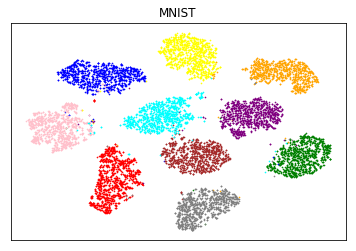
\includegraphics{embeddings_visualisation.png}
	\caption{Test point embedding using t-SNE}
\end{figure}

\small

\bibliography{bib}
\bibliographystyle{unsrt}


\end{document}
